\scanpage{123}
% archive foliation: 122
Un argument \unsure{assez} formel montre que
\[
\Gamma(F^\natural)\simeq\underset{H_\alpha}{\varinjlim}\ F^\natural(C_\alpha,G_\alpha)
\]
\deleted{où $\unsure{G_\alpha},C_\alpha$}
où $H_\alpha$ parcourt les sous-groupes \uline{inv} d’indice fini du groupe cartographique orienté, $C_\alpha$ est la carte orientée associée à $H_\alpha$, $G_\alpha=\mathbb G_2^+/H_\alpha$.
\uline{Ex} Soit $F(C)=\mathcal P(X)$, alors
\[
\Gamma F^\natural\simeq\mathcal P(S)/\operatorname{Aut}^\circ(S,
\]
$S$ \unsure{est} la sphère munie du segment $[0,1]$ et du point $\infty$,
\deleted{\unsure{pointée en $(0,1,\infty)$}} qui sert de référence dans notre théorie de cartographie.
\figure{\begin{tikzpicture}[scale=.8]
\draw(0,0)ellipse(1.2 and1.3);\draw[dashed](-1.2,0)..controls(-.4,.6)and(.5,.6)..(1.2,.15);
\draw[dashed](-1.2,0)..controls(-1,-.35)..(-.7,-.3);
\draw[very thick](-.7,-.3)..controls(.4,-.4)..(1.2,.15);
\draw(-.7,-.3)..controls(-.4,.2)and(.3,.3)..(1.2,.15);
\fill(-.7,-.3)circle(2pt)node[below]{$0$};\fill(1.2,.15)circle(2pt)node[right]{$1$};\fill(0,.4)circle(2pt)node[right]{$\infty$};
\end{tikzpicture}}
\uline{NB} Si on avait pris la théorie non orientée, on aurait trouvé
\[
\Gamma(F^\natural)\simeq\mathcal P(S)^{\uline c}/
\underbrace{\operatorname{Aut}(S,\uline c,0,1,\infty)^\circ}_{\simeq\operatorname{Aut}(S^+,0,1,\infty)^\circ}
\]
où $\uline c$ est la conjugaison (ayant comme pts fixes l’``équateur'' qui passe par $0,1,\infty\ldots$)
\uline{NB} On prouve \inserted{\unsure{aussitôt}} que, pour que \deleted{\unsure{notre}}\inserted{la} section $\Omega$ de $F^\natural$ \deleted{\unsure{associée}}\inserted{définie}: une partie \inserted{$A$} de $S$ \deleted{définie}\inserted{associe} \deleted{\unsure{, puis à}} à toute carte $C=(X,K,S)$ \deleted{des} parties \inserted{$A_X$} de $X$ qui \deleted{\unsure{sont}} un sous-$1$-complexe topologique, il f. et s. que la partie de $S$ envisagée soit de $=$ \unsure{nature}.
\figure{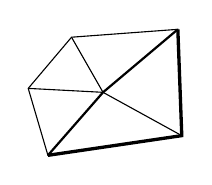
\begin{tikzpicture}
\draw(0,0)--(1.7,.25)--(1.65,1.6)--(.3,1.5)--(-.25,.85)--cycle;
\draw[thick](0,0)--(.7,.8)--(1.65,1.6);\draw(.3,1.5)--(.7,.8)--(1.7,.25);\draw(-.25,.85)--(.7,.8);
\draw[very thick](0,0)--(1.7,.25)--(1.65,1.6);\end{tikzpicture}}
Pour que les $A_X\cup K$ soient des sous-$1$-complexes (pas de \unsure{somm.-gén.|somm. qui}) \unsure{cf] et 1|si] et 1}.
